\documentclass[border={0.1cm 0.25cm 0.1cm 0.25cm}]{standalone}  %E,S,W,N

\usepackage{amssymb}
\usepackage{amsmath}
\usepackage{tikz}

% Note:	This is partly an experiment in making nodes & curves automatically adjustable
%		First, the size is adjustable (\x), as well as where the angle starts (\c% through the line)
%		The nodes will mostly adjust on their own to changes in size, as will the handle & curves
%		Big changes (e.g. \x=8) require changing the textsize (e.g. \small), and updating the xshift

\begin{document}
	
	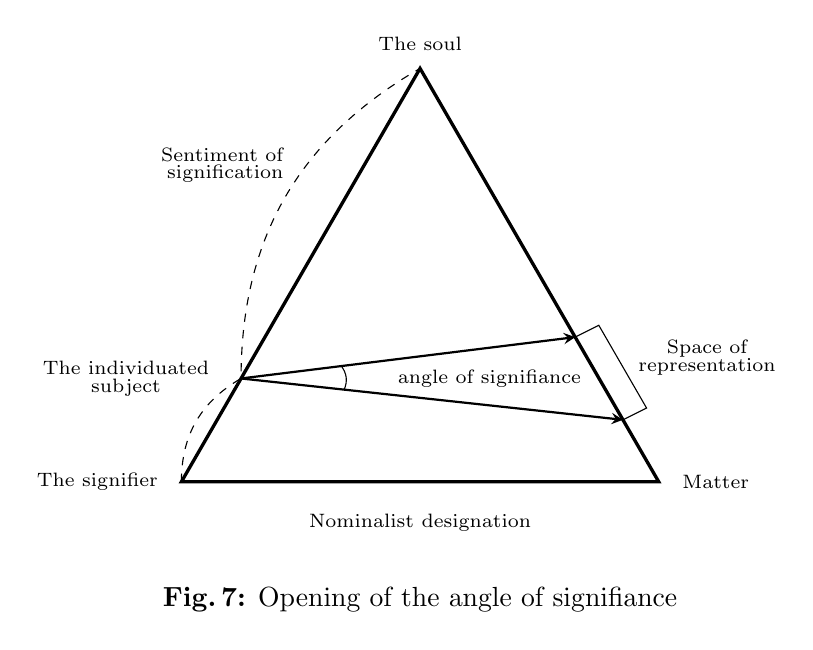
\begin{tikzpicture}	
	\def\x{3.5} %length of main circle	\draw[red] (0,0) circle (\x cm);	
	\def\c{0.25} %proportion on left side where the arrows begin
	
	%TRIANGLE
	\draw[very thick] ({-0.5*sqrt(3)*\x},-\x/2)--({0.5*sqrt(3)*\x},-\x/2)--(0,\x)--cycle;
	
	%ARROWS
	\draw[thick,->,>=stealth] ({(1-\c)*-0.5*sqrt(3)*\x},{-\x/2+1.5*(\c)*\x})-- ({(1-\c-0.1)*0.5*sqrt(3)*\x},{-\x/2+1.5*(\c+0.1)*\x}); %top arrow
	\draw[thick,->,>=stealth] ({(1-\c)*-0.5*sqrt(3)*\x},{-\x/2+1.5*(\c)*\x})-- ({(1-\c+0.1)*0.5*sqrt(3)*\x},{-\x/2+1.5*(\c-0.1)*\x}); %bottom arrow
	\draw ({(1-\c-0.1)*0.5*sqrt(3)*\x},{-\x/2+1.5*(\c+0.1)*\x})--++({(3/35)*\x},{(3/70)*\x})-- ({(1-\c+0.1)*0.5*sqrt(3)*\x+(3/35)*\x},{-\x/2+1.5*(\c-0.1)*\x+(3/70)*\x})-- ++({(-3/35)*\x},{(-3/70)*\x}); %handle
	
	%CURVED LINES
	\draw[dashed] ({-0.5*sqrt(3)*\x},-\x/2) to[bend left] ({(1-\c)*-0.5*sqrt(3)*\x},{-\x/2+1.5*(\c)*\x}) to[bend left] (0,\x); %dashed lines
	%
	\def\n{0.3} %position of angle curve
	\draw ({(1-\n)*((1-\c)*-0.5*sqrt(3)*\x)+\n*(1-\c-0.1)*0.5*sqrt(3)*\x}, {(1-\n)*(-\x/2+1.5*(\c)*\x)+\n*(-\x/2+1.5*(\c+0.1)*\x)}) to[bend left] ({(1-0.9*\n)*((1-\c)*-0.5*sqrt(3)*\x)+(0.9*\n)*(1-\c+0.1)*0.5*sqrt(3)*\x}, {(1-0.9*\n)*(-\x/2+1.5*(\c)*\x)+(0.9*\n)*(-\x/2+1.5*(\c-0.1)*\x)});
	%to get 1/n the length of a line, weight as x = (1-1\n)x_1 + (1/n)x_2
	
	%LABELS
	\node[above,yshift=3pt] at (0,\x) {\scriptsize The soul};
	\node[align=right,left,xshift=-5pt] at ({-0.5*sqrt(3)*\x},-\x/2) {\scriptsize The signifier};
	\node[right,xshift=5pt] at ({0.5*sqrt(3)*\x},-\x/2) {\scriptsize Matter};
	\node[align=center,left,xshift=-8pt] at ({(1-\c)*-0.5*sqrt(3)*\x},{-\x/2+1.5*(\c)*\x}) {\scriptsize The individuated\\[-2mm]\scriptsize subject};
	\node[align=center,right,xshift=15pt] at ({(1-\c-0.05)*0.5*sqrt(3)*\x},{-\x/2+1.5*(\c+0.05)*\x}) {\scriptsize Space of\\[-2mm]\scriptsize representation};
	\node[align=right,left,xshift=-3pt] at ({(1-\c)*0.5*sqrt(3)*\x},{-\x/2+1.5*(\c)*\x}) {\scriptsize angle of signifiance};
	\def\s{0.6} %position of label
	\node[align=right,above left,xshift=-20pt] at ({(1-\s)*((1-\c)*-0.5*sqrt(3)*\x)+\s*(0)}, {(1-\s)*(-\x/2+1.5*(\c)*\x)+\s*(\x)}) {\scriptsize Sentiment of\\[-2mm] \scriptsize signification};
	\node[below,yshift=-8pt] at (0,-\x/2) {\scriptsize Nominalist designation};
	%
	\node at (0,-\x/2-1.5) {\textbf{Fig.$\,$7:} Opening of the angle of signifiance};
	\end{tikzpicture}
	
\end{document}